A secondary focus of this thesis is to transform the parsed dataset into an easily interpretable, and information rich
knowledge graph to server further downstream research as part of MEHDIE~\cite{MEHDIE}.

To create such a graph, it is beneficial to rely on existing ontologies, to increase inter-compatibility and standardization.
Specifically, this new Kitāb KG's ontology extends Wikidata's ontology in terms of relationship and category types.

In terms of place node ontology however, the KG was constructed by entirely using internal ids.

As mentioned earlier in section TODO, some Wikidata equalency information was already available in the parsed dataset.
This information was also used to expand the graph, and moreover, could potentially be used to help training better models for link prediction.

\subsection{Hierarchical Edges}
While there are no concrete rules for knowledge graph constructions, one could take two different approaches.
Either the graph could explicitly contain all known hierarchical edges (figure~\ref{fig:kg-dense}),
or just the next level up in the hierarchy (figure~\ref{fig:kg-comp}).

It seems that the larger well-known graphs do not explicitly define all levels of hierarchy for any given place.
Therefore, this knowledge graph was also constructed in a compositional manner.

\begin{figure}[h] % [h] attempts to place figure here, other options like [t]op, [b]ottom
    \centering % Centers the figure horizontally
    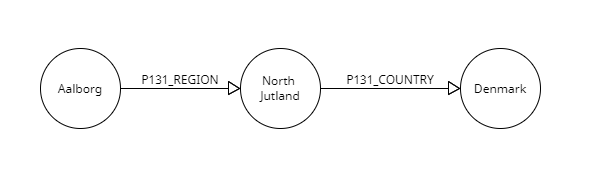
\includegraphics[width=0.9\linewidth]{figures/kg-comp} % Include the image with desired width
    \caption{Small example of a graph where not all known hierarhical relationships are defined} % Add a caption
    \label{fig:kg-comp} % Assign a label for referencing the figure in text
\end{figure}

\begin{figure}[h] % [h] attempts to place figure here, other options like [t]op, [b]ottom
    \centering % Centers the figure horizontally
    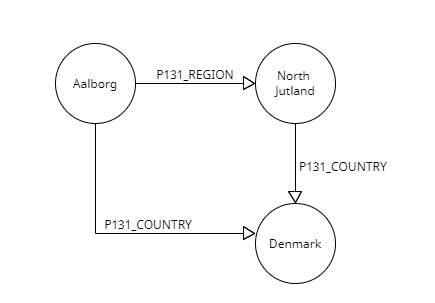
\includegraphics[width=0.7\linewidth]{figures/kg-dense} % Include the image with desired width
    \caption{Small example of a graph where all known hierarhical relationships are explicitly defined} % Add a caption
    \label{fig:kg-dense} % Assign a label for referencing the figure in text
\end{figure}

Another caveat is that Wikidata's ontology does not define various hierarhical-edge types, and instead relies on
the aggregating P131 edge type (located in the administrative territorial entity).

For the purposes of this KG, it is more beneficial to split this type into three distinct types, namely:
\textbf{wd\_P131\_METROPOLITAN}, \textbf{wd\_P131\_DISTRICT} and \textbf{wd\_P131\_PROVINCE}


\subsection{Distance Edges}
In the parsed Kitāb dataset there is a large amount of distance information between various place pairs.
However, just simply inserting these edges into the KG,
without the numerical distance values would significantly diminish the informational value of the graph.

However, the simple triplet structure of knowledge graphs do not the definition features on edges or nodes.
Normally, the place nodes would have a corresponding point literal in the triplet store, and the distance
between the two points could be extracted using some geospatial calculation.

Unfortunately, in this case there are very few nodes with known coordinates.
As a compromise, the \textbf{Distance} edge types was split into multiple edge types, each
type representing a specific range.

These binned edge types are also shown on table:~\ref{tab:kg-edges}

Finally, as the distance is obviously symmetric, these triplets were defined twice by switching the head and tail
entities.

\subsection{Categories}
There is a significant overlap between the categories defined in the parsed Kitāb dataset and the available
conceptual entities in Wikidata, wherever available, the Wikidata Ontology Id was used.

For example, the city category was mapped to the Wikidata entity \textit{Q515}.
However, there were some very specific categories in the parsed dataset, such
as kasbah (city center) which is distinct from just a generic kasbah \textit{Q89468}

These special category entities were defined in the Mehdie ontology.
E.g kasbah (city center) became \textit{Q89468}

Since the categories are hierarchical, this hierarchy was captured using the \textbf{P279}
(subclass of) edge type, with the place nodes referencing the lowest available category level.
Between Place and Category entities, the \textbf{P31} edge type was used.

\subsection{Scraping Wikidata}
As mentioned earlier, in the parsed Kitāb dataset, a number of places had a Wikidata Id defined.
This introduced the opportunity to enrich the knowledge graph with extra wikidata information.

The full list of scraped edge types are listed on table~\ref{tab:kg-edges}

One could make the argument that if a Place node has a corresponding Wikidata entity,
then it is bad practice to keep both nodes in the graph.

However, considering that these ID assignments may be incorrect, it is safer to link the corresponding
MEHDIE and Wikidata entities with a \textbf{P460} - "said to be the same as".

\begin{table}[!ht]
    \centering
    \caption{Edge types used in the Kitāb Knowledge Graph}
    \begin{tabular}{|l|l|}
        \hline
        Name & Description \\ \hline
        \textbf{wd\_P131\_METROPOLITAN} & \textit{head} is in the metropolitan area of \textit{tail}\\ \hline
\textbf{wd\_P131\_DISTRICT} &  \textit{head} is in the district area of \textit{tail} \\ \hline
\textbf{wd\_P131\_PROVINCE} & \textit{head} is in the provincial area of \textit{tail} \\ \hline
\textbf{DISTANCE\_0\_5} & \textit{head} and \textit{tail} are closer than 5km to each other \\ \hline
\textbf{DISTANCE\_5\_10} & \textit{head} and \textit{tail} are between 5 and 10 kilometers from each other \\ \hline
\textbf{DISTANCE\_10\_20} & \textit{head} and \textit{tail} are between 10 and 20 kilometers from each other \\ \hline
\textbf{DISTANCE\_20\_50} & \textit{head} and \textit{tail} are between 20 and 50 kilometers from each other \\ \hline
\textbf{DISTANCE\_100\_200} & \textit{head} and \textit{tail} are between 100 and 200 kilometers from each other \\ \hline
\textbf{DISTANCE\_200\_500} & \textit{head} and \textit{tail} are between 200 and 500 kilometers from each other \\ \hline
\textbf{DISTANCE\_500\_1000} & \textit{head} and \textit{tail} are between 500 and 1000 kilometers from each other \\ \hline
\textbf{DISTANCE\_1000\_inf} & \textit{head} and \textit{tail} are over 1000 km away from each other \\ \hline
\textbf{P17} & Wikidata type: "Country" \\ \hline
\textbf{P206} & Wikidata type: "located in or next to body of water" \\ \hline
\textbf{P706} & Wikidata type: "located in/on physical feature" \\ \hline
\textbf{P361} & Wikidata type:  "part of" \\ \hline
\textbf{P402} & Wikidata type: "OpenStreetMap relation ID" \\ \hline
\textbf{P11693} & Wikidata type:  "OpenStreetMap node ID" \\ \hline
\textbf{P625} & Wikidata type: "coordinate location" \\ \hline
\textbf{P460} & Wikidata type: "said to be the same as" \\ \hline
\end{tabular}
\label{tab:kg-edges}
\end{table}